\begin{figure}[ht]
    \centering
    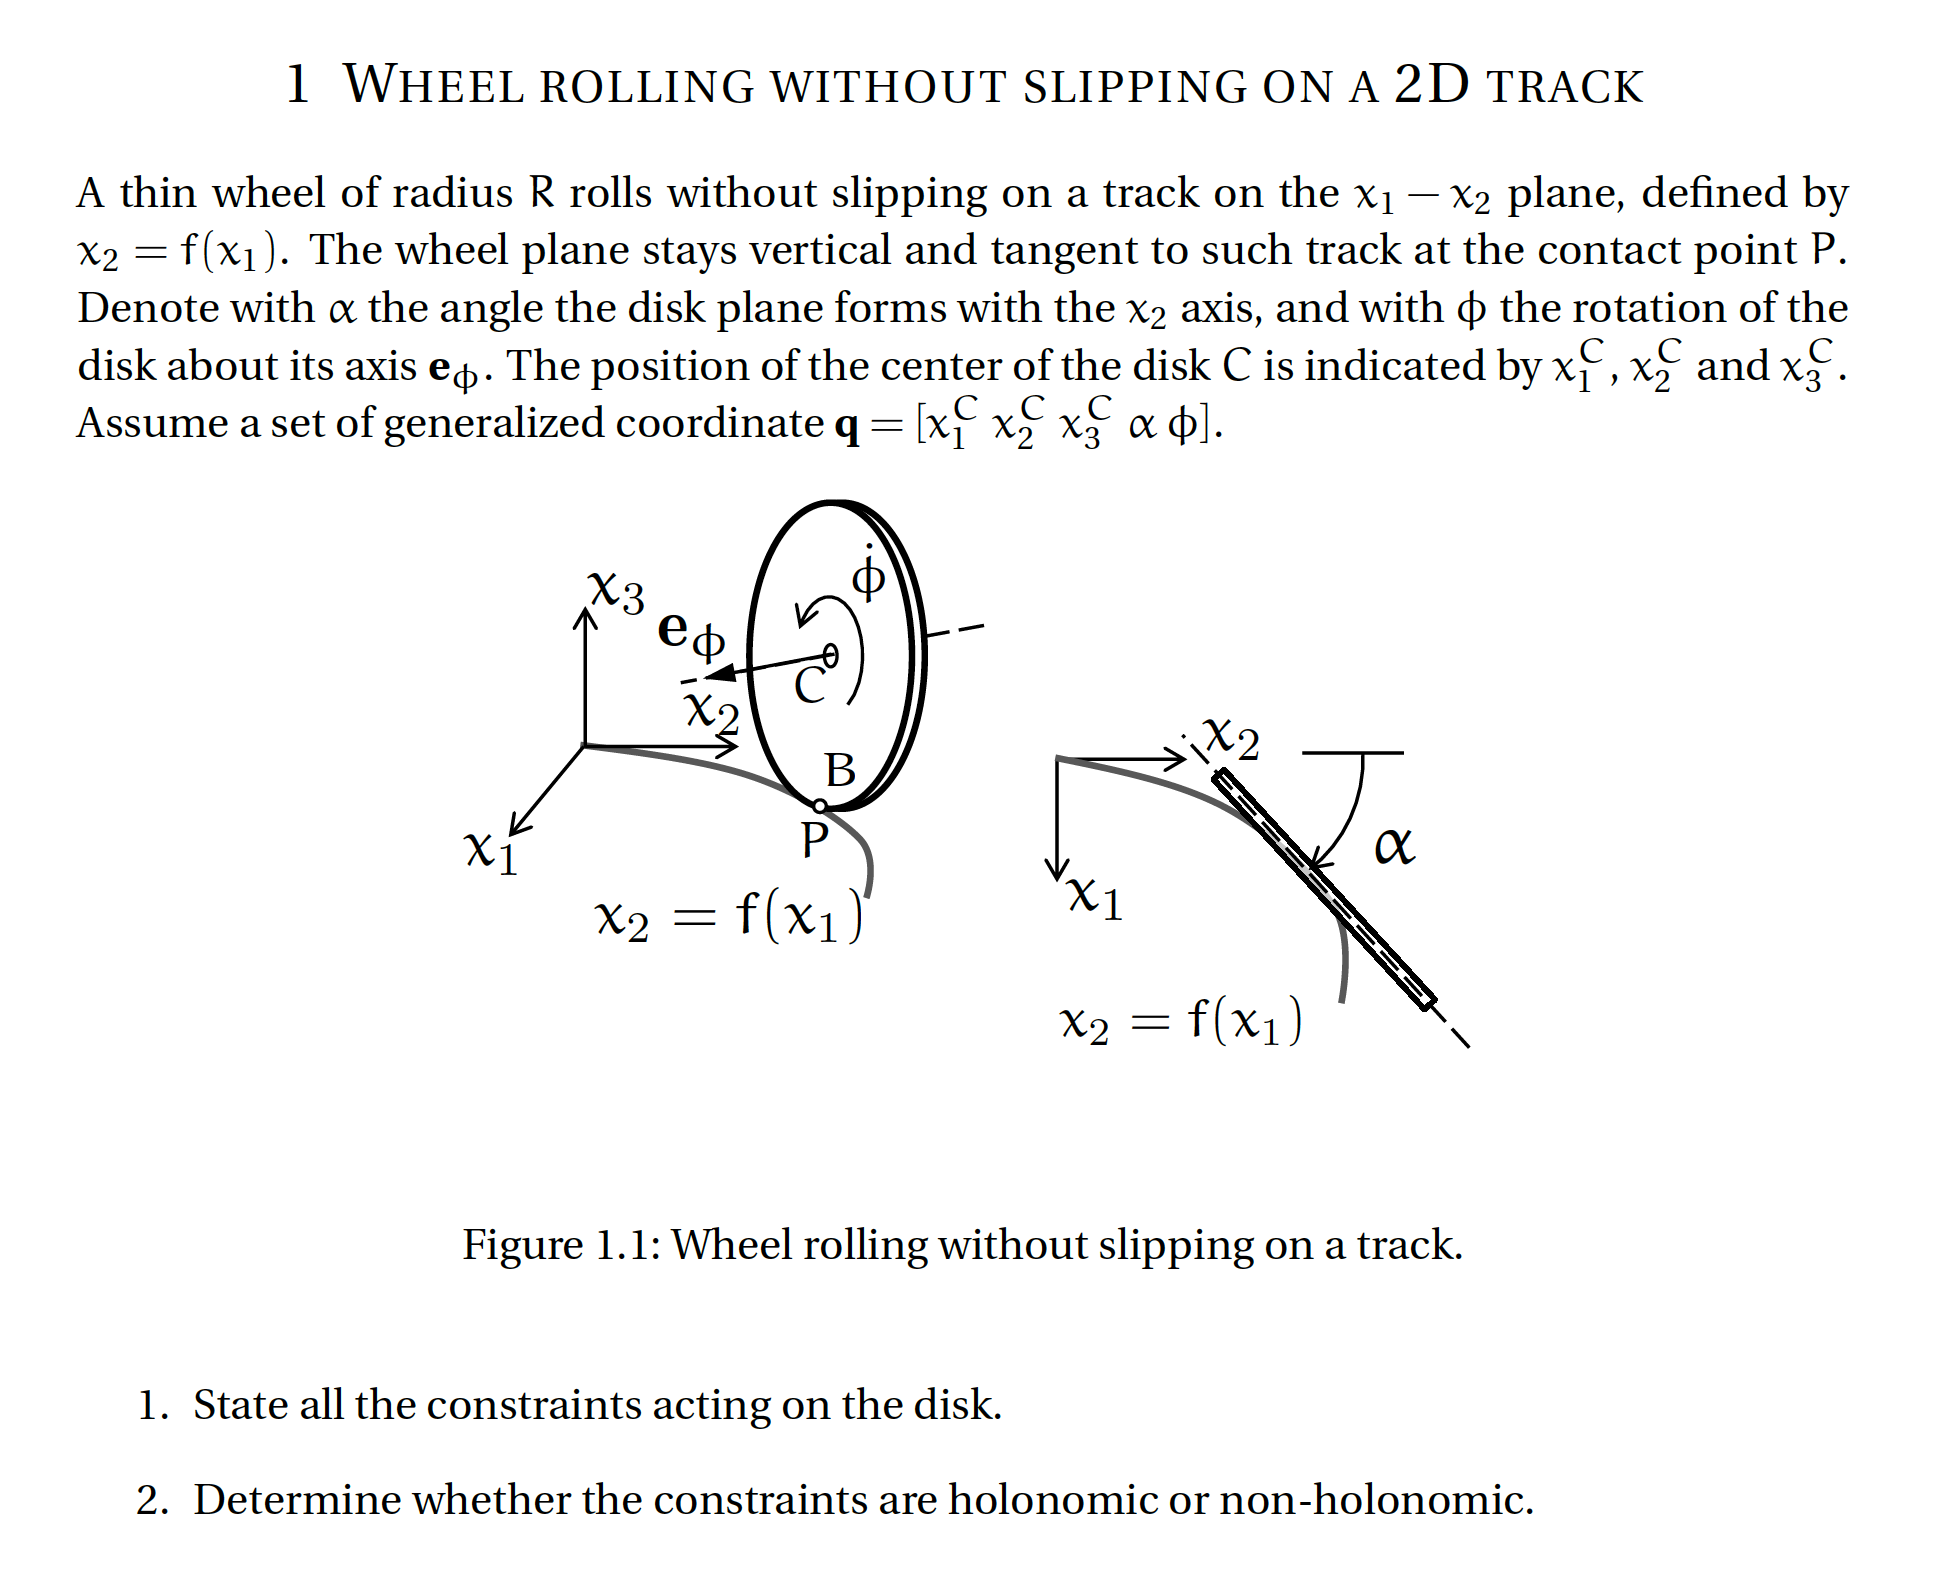
\includegraphics[scale=0.4]{images/1.1.png}
    \caption{Task 1.1}
    %label always in the end
    \label{fig:task1.1}
\end{figure}
\clearpage

\subsection{}
\subsubsection{}\label{subsubsec:1.1.1}
The list of constraints looks as follows:

\begin{enumerate}
    \item The wheel always stays vertical (plane parallel to $x_3$)\\
        This is a holonomic constraint: $f = \theta = 0$ where $\theta$ denotes the angle between the disk and $x_3$
    \item $x_2$ follows a fixed trajectory, given $x_1$ (and vice versa):\\
        $f_2: x_2 = f(x_1) \Rightarrow x_2 - f(x_1) = 0 \Rightarrow$ holonomic.
    \item $\alpha$ is the angle between the trajectory and the $x_2$ axis:\\
        $\alpha = \frac{\pi}2 - \frac{\partial f(x_1)}{\partial x_1}$ or written differently:\\
             $f(\alpha, x_1) = \alpha - \frac{\pi}2 + \frac{\partial f(x_1)}{\partial x_1} = 0 \Rightarrow$ holonomic
    \item Rolling without slipping:\\
        $v^B = 0 \Rightarrow v_C + \omega \times R_{CB} = 0$ with $\omega = \dot{\alpha}\boldsymbol{e_3} + \dot\phi\boldsymbol{e_\phi}$\\
        Seems to be non-holonomic at first glance
    \item The disk does not leave the ground:\\
        $x_3^C - R = 0$ aka the $x_3$ component of the center of mass is R.\\
        This is holonomic as well
\end{enumerate}

\noindent So far we have a 3D system (6 DoF) and 4 holonomic constraints and 1 non-holonomic constraint.\vspace{1cm}

4. Check for integrability:
\begin{equation}
    \begin{split}
        &v^B = 0 \Rightarrow v_C + \omega \times R_{CB} = 0\\
    \end{split}
\end{equation}
Plugging in $\dot{x}_1^C, \dot{x}_2^C, \omega = \dot{\alpha}\boldsymbol{e_3} + \dot\phi\boldsymbol{e_\phi} \text{ and } R_{CB} = [0,0,-R]^T$:
\begin{equation}
    \begin{split}
        &\dot x_1^C\boldsymbol{e_1} + \dot x_2^C\boldsymbol{e_2} -  R\dot\phi\cos\alpha\boldsymbol{e_2} - R\dot\phi\sin\alpha\boldsymbol{e_1} = 0
    \end{split}
\end{equation}

Considering the part in $\boldsymbol{e_1}$ direction:
\begin{equation}\label{eq:1.3}
    \begin{split}
        &\dot x_1^C - R\dot\phi\sin\alpha = 0 
    \end{split}
\end{equation}

As $\alpha$ is not dependent on time it can be easily seen that \ref{eq:1.3} is integrable:

\begin{equation}\label{eq:1.4}
    \begin{split}
        &\int\dot x_1^Cdt = \int R\dot\phi\sin\alpha dt\\
        &\Rightarrow x_1^C = R\phi\sin\alpha
    \end{split}
\end{equation}

% Now if we reformulate this in the linear velocity form:
% \begin{equation}
%     \sum_{i=1}^n a_i(\boldsymbol{q},t)\dot q_i + b(\boldsymbol{q},t) \text{ with \textbf{q} = }[x_1^C,x_2^C, x_3^C,\alpha, \phi]
% \end{equation}
% We get
% \begin{equation}
%     \begin{split}
%         &a_1 = 1, \quad a_5 = -R\sin(\alpha), b = 0\\
%         &\Rightarrow \frac{\partial(Cb)}{\partial q_1} = \frac{\partial(Ca_1)}{\partial t} \Rightarrow \frac{\partial C}{\partial t} = 0 \Rightarrow C \neq C(t)\\
%         &\Rightarrow \frac{\partial(Ca_1)}{\partial q_5} = \frac{\partial(Ca_5)}{\partial q_1} \Rightarrow \frac{\partial(C)}{\partial \phi} = \frac{\partial(-CR\sin(\alpha))}{\partial x_1^C}\\
%         & \Rightarrow \frac{\partial(C)}{\partial \phi} = -R\sin(\alpha)\frac{\partial(C)}{\partial x_1^C}
%     \end{split}
% \end{equation}
% Perhaps we can show directly that the constraint can be written in the solution form:
% \begin{equation}
%     \begin{split}
%         \dot x_1^C\boldsymbol{e_1} - R\dot\phi\sin\alpha\boldsymbol{e_1} = \sum_{i=1}^n \frac{\partial f(\boldsymbol{q},t)}{x_1^C}\dot x_1^C + \frac{\partial f(\boldsymbol{q},t)}{\phi}\dot \phi
%     \end{split}
% \end{equation}
\subsubsection{}
See subsubsection \ref{subsubsec:1.1.1}
\subsubsection{}

\begin{figure}[ht]
    \centering
    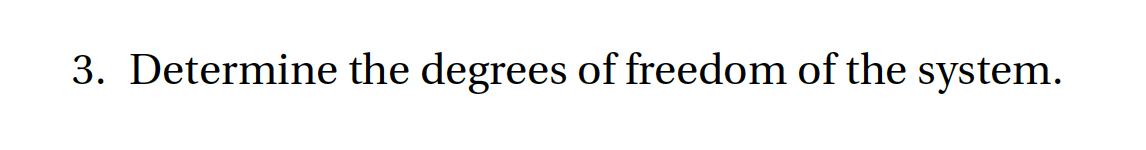
\includegraphics[scale=0.4]{images/1.1.3.png}
    \caption{Task 1.1.3}
    %label always in the end
    \label{fig:task1.1.3}
\end{figure}

\noindent As we have a 3D body with 6 generalized coordinates (here 5 are given, already considering constraint 1) and 5 holonomic constraints. We get a total of $6 - 5 = 1$ degree of freedom. That could for instance be the rotation of the wheel around $\boldsymbol{e_\phi}$ while all the other generalized coordinates follow accordingly.

\clearpage

\begin{figure}[ht]
    \centering
    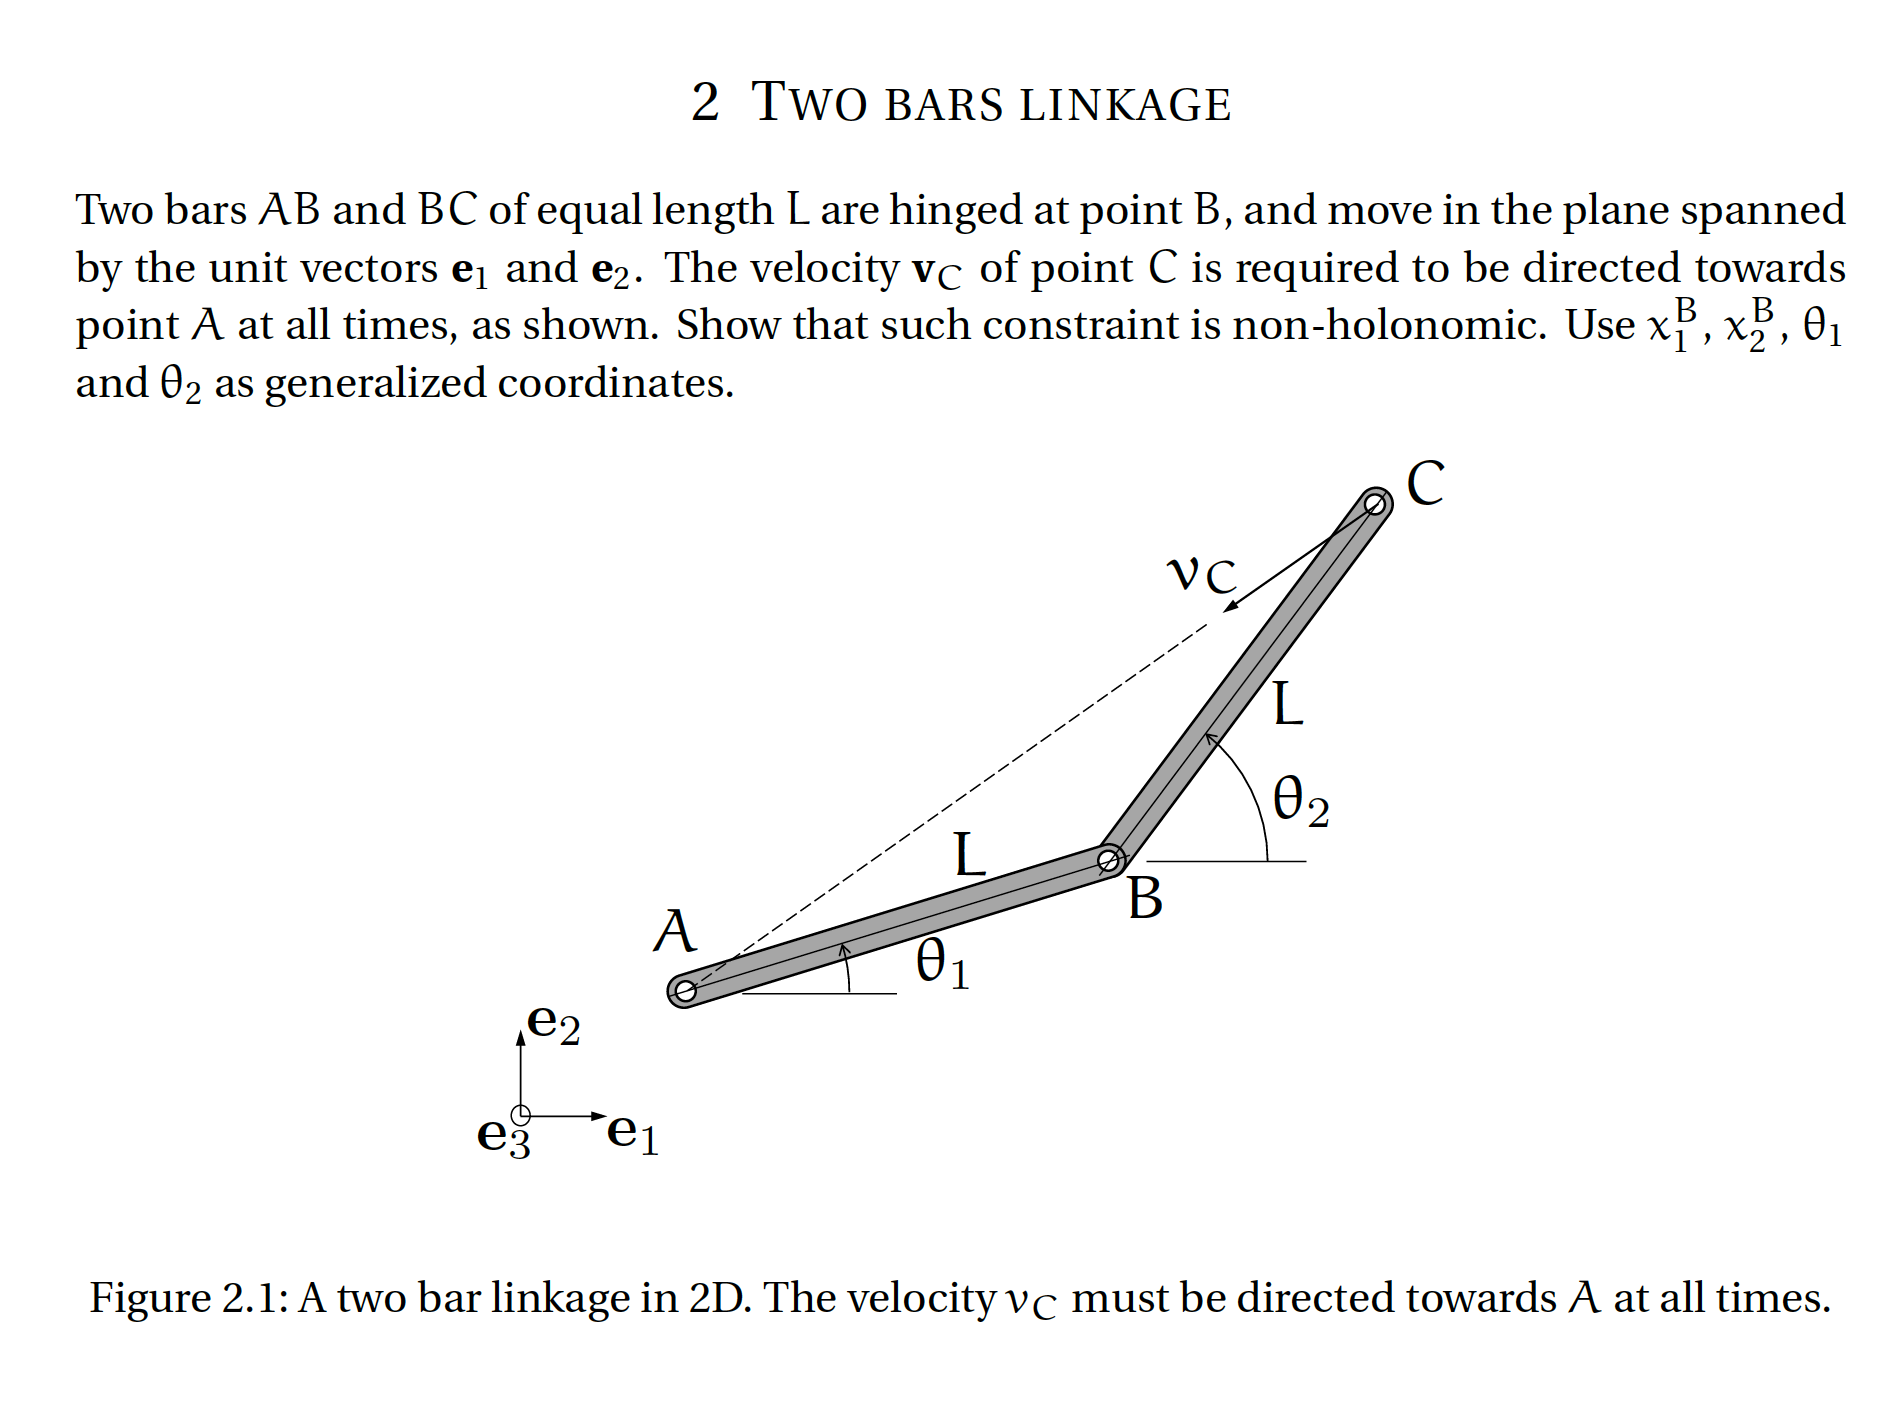
\includegraphics[scale=0.4]{images/1.2.png}
    \caption{Task 1.1}
    %label always in the end
    \label{fig:task1.2}
\end{figure}
\subsection{}\label{subsec:1.2}

I want to show that the constraint that $v_c$ always points in the direction of $AD$ is not integrable. I would like to express this constraint as:
\begin{equation}
    \begin{split}
        &v_C * AC_p = 0 \\
        &\text{where }AC_p \text{ is a vector
         perpendicular to }AC
    \end{split}
\end{equation} 

The velocity of point C can be found either by expressing the position of C and derivating or using the velocity transfer formula from B to C which yields:

\begin{equation}
    \begin{split}
        v_C = \begin{pmatrix}
            \dot x_1^B - L\sin(\theta_2)\dot\theta_2\\
            \dot x_2^B + L\cos(\theta_2)\dot\theta_2
        \end{pmatrix}
    \end{split}
\end{equation}

And AC is simply:
\begin{equation}
    \begin{split}
        AC = \begin{pmatrix}
            L\left(\cos\theta_1+\cos\theta_2\right)\\L\left(\sin\theta_1+\sin\theta_2\right)
        \end{pmatrix}
    \end{split}
\end{equation}

A simple vector that is perpendicular to AC can be gotten by switching the $e_1$ and $e_2$ entries and switching the sign of one of them:

\begin{equation}
    \begin{split}
        AC_p = \begin{pmatrix}
            L\left(\sin\theta_1+\sin\theta_2\right)\\
            -L\left(\cos\theta_1+\cos\theta_2\right)
        \end{pmatrix}
    \end{split}
\end{equation}

\begin{equation}
    \begin{split}
        \Rightarrow &v_C * AC_p =
        \begin{pmatrix}
            \dot x_1^B - L\sin(\theta_2)\dot\theta_2\\
            \dot x_2^B + L\cos(\theta_2)\dot\theta_2
        \end{pmatrix} * \begin{pmatrix}
            L\left(\sin\theta_1+\sin\theta_2\right)\\
            -L\left(\cos\theta_1+\cos\theta_2\right)
        \end{pmatrix} = \\
        &\left(L\left(\sin\left(\theta _1\right)+\sin\left(\theta _2\right)\right)\right)\mathrm{\dot x_1}^B+\left(-L\left(\cos\left(\theta _1\right)+\cos\left(\theta _2\right)\right)\right)\dot x_2^B-\\
        &L^2\dot\theta_2\cos\left(\theta _2\right)\left(\cos\left(\theta _1\right)+\cos\left(\theta _2\right)\right)-L^2\dot\theta_2\sin\left(\theta _2\right)\left(\sin\left(\theta _1\right)+\sin\left(\theta _2\right)\right) = 0
    \end{split}
\end{equation} 

After applying trigonometry:

\begin{equation}
    \begin{split}           
        &\left(L\left(\sin\left(\theta _1\right)+\sin\left(\theta _2\right)\right)\right)\mathrm{\dot x_1}^B+\left(-L\left(\cos\left(\theta _1\right)+\cos\left(\theta _2\right)\right)\right)\dot x_2^B-\\
        &L^2\dot\theta_2\left(\cos\left(\theta _2\right)\cos\left(\theta _1\right)+\sin\left(\theta _2\right)\sin\left(\theta _1\right)+1\right) = 0
    \end{split}
\end{equation}

To simplify the notation I will refer to $\sin \theta_1$ as $s_1$ and $\sin \theta_2$ as $s_2$:

\begin{equation}
    \begin{split}           
        &L\dot x_1^B\left(s_1+s_2\right)-L\dot x_2^B\left(c_1+c_2\right)-
        L^2\dot\theta_2^2\left(c_2c_1+s_2s_1 + 1\right) = 0
    \end{split}
\end{equation}

Dividing by L:

\begin{equation}
    \begin{split}           
        &\dot x_1^B\left(s_1+s_2\right)-\dot x_2^B\left(c_1+c_2\right)-
        L\dot\theta_2^2\left(c_2c_1+s_2s_1 + 1\right) = 0
    \end{split}
\end{equation}

With the generalized coordinates $q = [x_1^B,x_2^B,\theta_1,\theta_2]$

Writing down the coefficients of the non-holonomic constraint:

\begin{equation}
    \begin{split}
        &a_1 = s_1 + s_2\\
        &a_2 = -\left(c_1 + c_2\right)\\
        &a_3 = 0\\
        &a_4 = -L\left(1 + s_1s_2 + c_1c_2\right)\\
        &b = 0
    \end{split}
\end{equation}

\clearpage
To check for the exact velocity form we want to proof that there can't exist a $C(q) \neq 0$ for which holds:

\begin{equation}
    \begin{split}
        \frac{\partial(Cb)}{\partial q_i} = \frac{\partial(Ca_1)}{\partial t}\quad \text{ and } \quad \frac{\partial(Ca_i)}{\partial q_k} = \frac{\partial(Ca_k)}{\partial q_i} \quad \text{ for all the gen. coord. }
    \end{split}
\end{equation}

q1-q3:

\begin{equation}
    \begin{split}
        &\frac{\partial(Ca_1)}{\partial \theta_1} = 0 \Rightarrow C*c_1 + \frac{\partial C}{\partial \theta_1}(s1 + s2) = 0\\
        &\Rightarrow \frac{c_1}{s1+s2} + \frac{1}{C}\frac{d C}{d \theta_1} = 0 \Rightarrow \int \frac{1}{C}dC = - \int \frac{c_1}{s_1+s_2}d\theta_1\\
        &\Rightarrow lnC = \frac{D}{s_1+s_2} + D \Rightarrow C = \frac{D}{s_1+s_2} \quad \text{ where the integration const. D was updated}\\
        &\Rightarrow C = \frac{D(x_1^B,x_2^B,\theta_2)}{s1 + s2}
    \end{split}
\end{equation}

q1 - q4:

\begin{equation}
    \begin{split}
        \frac{\partial C a_1}{\partial \theta_2} = \underbrace{\frac{\partial C a_4}{\partial x_1^B}}_{0} = 0 \Rightarrow \frac{\partial D}{\partial \theta_2} = 0 \Rightarrow C = \frac{D(x_1^B,x_2^B)}{s1 + s2}
    \end{split}
\end{equation}

q1 - q2:

\begin{equation}
    \begin{split}
        &\frac{\partial C a_1}{\partial x_2^B} = \frac{\partial C a_2}{\partial x_1^B}\Rightarrow \frac{\partial C}{\partial x_2^B}\left(s_1+s_2\right) = \frac{\partial C}{\partial x_1^B}\left(c_1+c_2\right) \Rightarrow \frac{\partial C}{\partial x_2^B} = \frac{\partial C}{\partial x_1^B}\frac{c_1+c_2}{s_1+s_2}\\
        &\text{Remembering that } D = D(x_1^B,x_2^B) \Rightarrow D = const.\\
        & \Rightarrow C = \frac{D}{s_1 + s_2} \text{ where D const.}
    \end{split}
\end{equation}

q2 - q3:

\begin{equation}
    \begin{split}
        &\frac{\partial C a_1}{\partial x_2^B}  = 0 \Rightarrow D\frac{\partial\frac{
        (c_1+c_2)}{s_1+s_2}}{\partial \theta_1} = 0\\
        &D\frac{\partial \frac{c_1}{s_1+s_2}}{\partial\theta_1} = -\frac{Ds_1}{s_1+s_2} - \frac{Dc_1^2}{(s_1+s_2)^2} = -D\frac{s_1(s_1+s_2) - c_1^2}{(s_1+s_2)^2}
    \end{split}
\end{equation}

\begin{equation}
    \begin{split}
        &D\frac{\partial \frac{c_2}{s_1+s_2}}{\partial\theta_1} = -D\frac{c_1c_2}{(s_1+s_2)^2}
    \end{split}
\end{equation}

Which leads to:

\begin{equation}
    \begin{split}
        -D\frac{c_1^2 + s_1^2 + s_1s_2 + c_1c_2}{(s_1+s_2)^2} \overset{\text{!}}{=} 0
    \end{split}
\end{equation}

Which is a contradiction. Therefore this is a non-holonomic constraint.

